\chapter[Classification]{Classification}
\label{ch:classification}
\index{classification|(}

A \textit{supervised learning}\index{classification!supervised learning} algorithm ''observes some example input-output pairs and learns a function that maps from input to output'' \citep{russel2016}. Outputs from a supervised learning problem may be \textit{quantitative}\index{classification!quantitative} - involving discrete numerical values, or \textit{qualitative}\index{classification!qualitative} - with values within a particular class or label \citep{james2006}.

A classification problem can be tackled using a supervised learning algorithm, which will predict a qualitative output (the target class) from a given set of variables \citep{russel2016}. Classification initially involves the training stage, during which a model learns how certain inputs correspond to an output using the available \textit{training data}\index{classification!training data}. This is followed by testing of the model, wherein the \textit{testing data}\index{classification!testing data} is then used to evaluate the accuracy of the model.

When two classes are available as outputs of a classification problem, then this is called \textit{binary classification}\index{classification!binary classification} \citep{neelamegam2013}. On the other hand, multiclass classification is used to define problems in which the response variable constitutes of more than two classes \citep{aly2005}.

\section{Applications of Classification Problems}
\label{sec:applications}
\index{classification!classification problems applications}

Classification models may be built to predict several outcomes in different scenarios. For example, in the health sector, classification can be helpful in predicting whether a person is diagnosed with a particular medical condition or not, based on certain parameters related to experienced symptoms \citep{venkata2011,alzahani2015}.

Financial sectors may find classifications helpful when it comes to predicting whether a company is bankrupt or in good financial health \citep{moradi2012}. Moreover, they may apply classifiers to determine whether a bank should issue a loan to a customer \citep{thomas2000}.

Similar classification models may be constructed when adequate training data is available for a classifier to learn how certain inputs relate to a particular target output.

\section{Classification Algorithms}
\label{sec:algorithms}

Over the years, researchers have come up with several algorithms that aid in solving classification problems, or have applied such algorithms for predicting outcomes in several scenarios. Examples of such classification algorithms include Naive Bayes classifier, Decision Trees, Support Vector Machines (SVM) or K-Nearest Neighbors (KNN), amongst others \citep{neelamegam2013}.

\subsection{Decision Trees} \index{classification!decision trees}

This algorithm builds a tree-structured classification model (Figure~\ref{fig:classification-decisiontree}), in which the nodes of the tree represent the different features, branches between the nodes represent decisions (or rules), whilst the leaf nodes represent the resultant class \citep{rokach2007}.

\begin{marginfigure}
    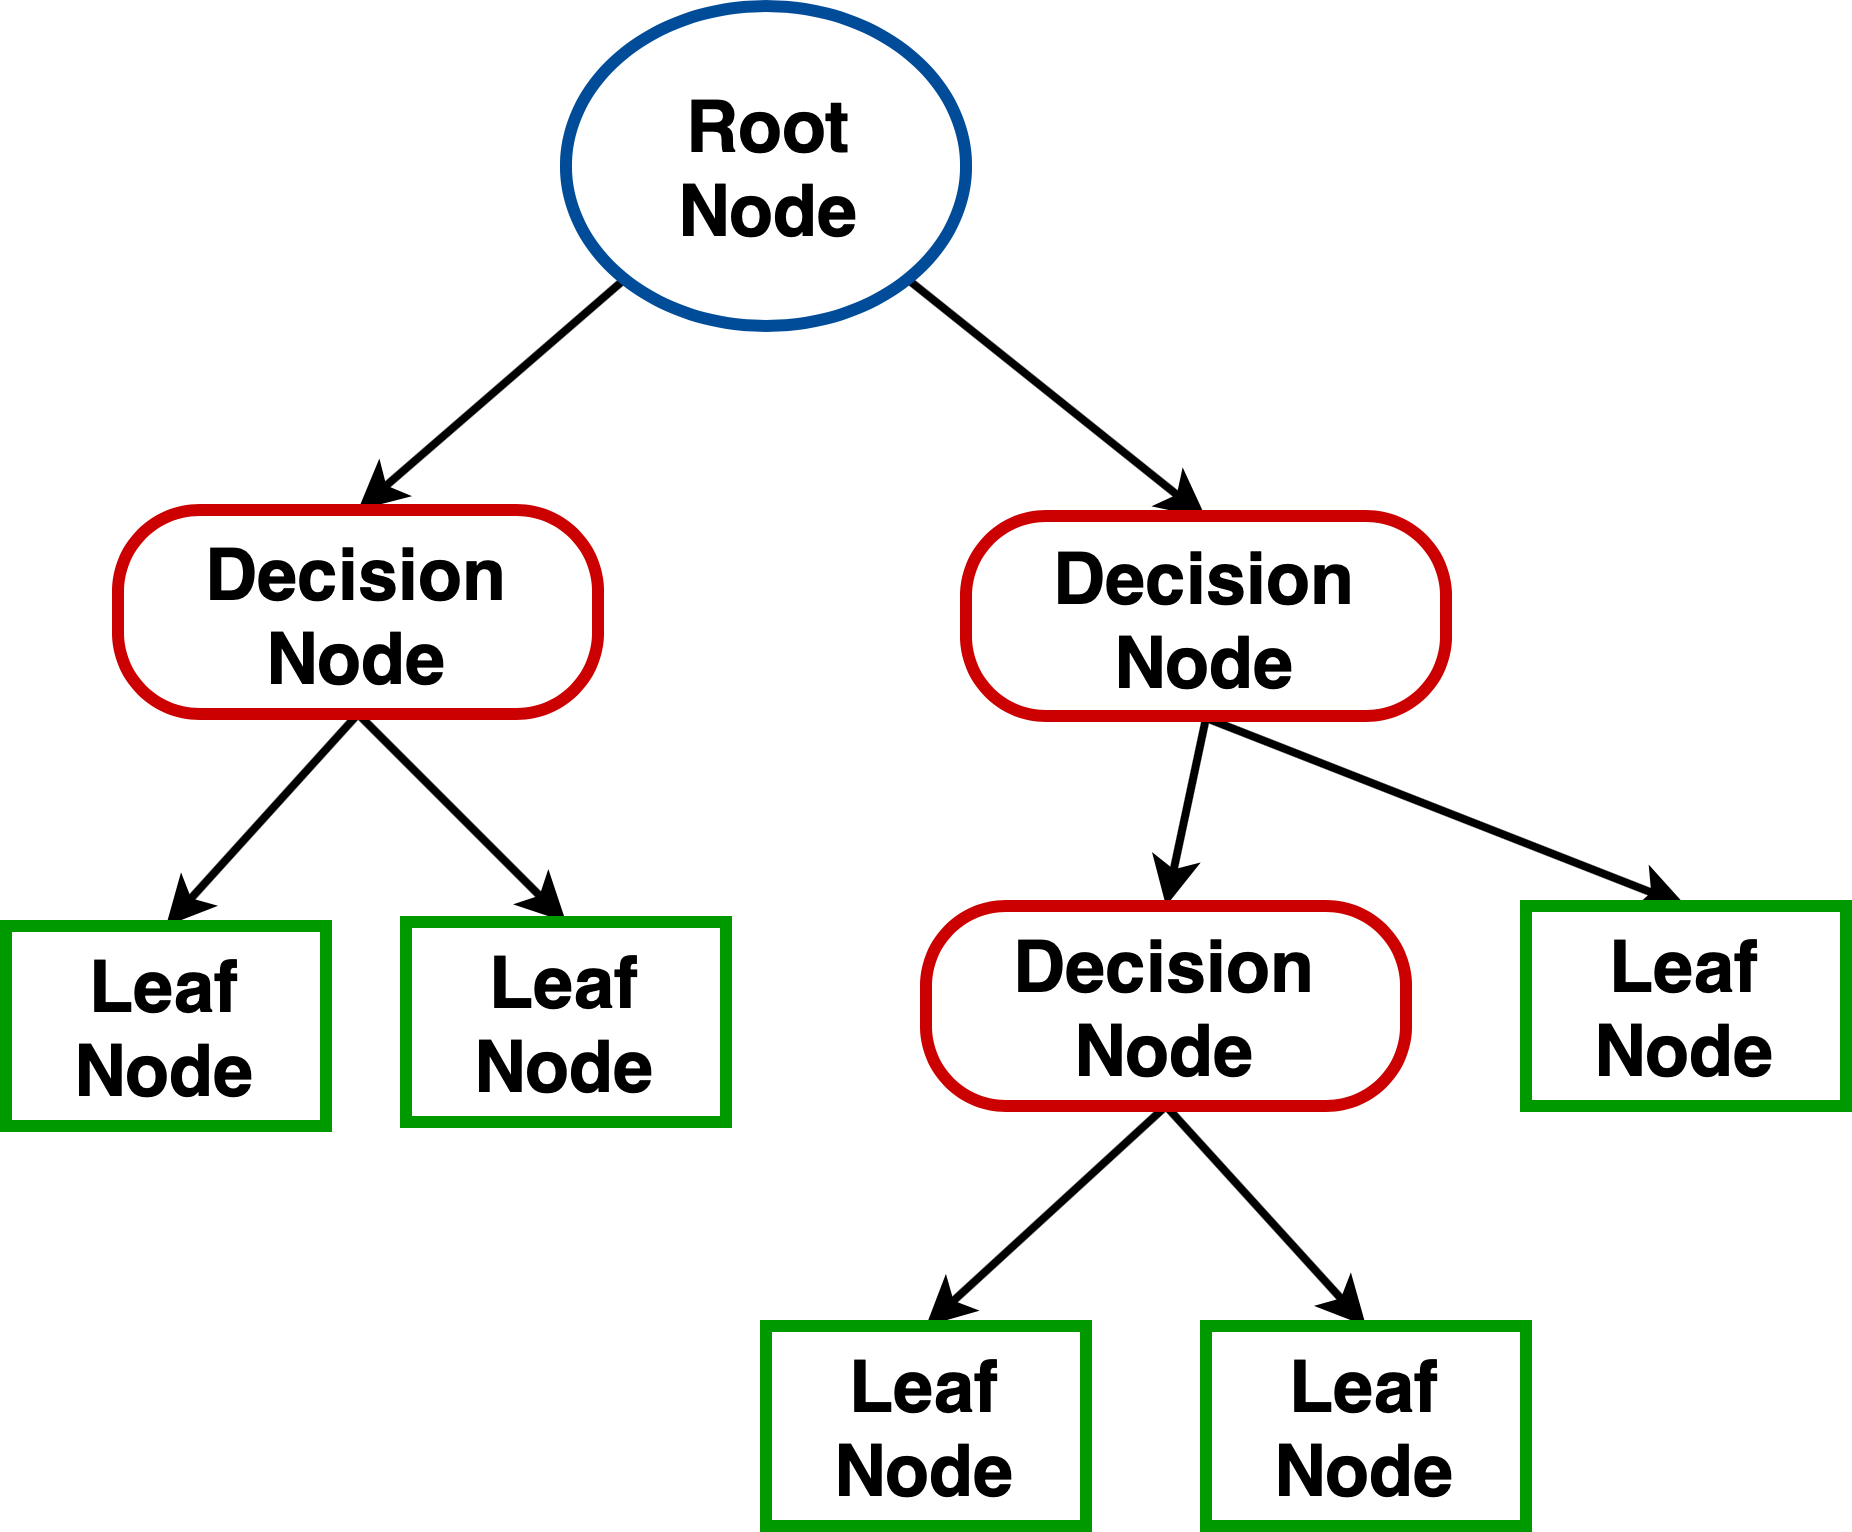
\includegraphics{graphics/classification/ClassificationDecisionTree.png}
    \caption{
    A representation of a decision tree.
    }
    \label{fig:classification-decisiontree}
\end{marginfigure}
Having adequate training data, a decision tree may be constructed using several algorithms, including \textit{Iterative Dichotomiser 3 (ID3)}\index{classification!decision trees!ID3} and \textit{Classification and Regression Trees (CART)}\index{classification!decision trees!CART} \citep{rokach2005}. Finding the optimal   decision tree entails a top-down recursive approach in which each iteration considers the feature with the highest importance and repeatedly splits the tree based on a splitting condition. Once the tree is constructed, pruning may be applied to obtain a more accurate decision tree which is generally smaller in size. \citet{rokach2005} further discuss splitting functions and pruning methods which may be used during decision tree induction.

To predict an outcome using the tree model, the algorithm starts from the root node of the tree and repeatedly traverses branches based on the feature values, until a leaf node is reached \citep{rokach2007}.

\subsection{Naive Bayes} \index{classification!naive bayes}

Naive Bayes classifiers are nowadays applied by Gmail and within other spam filtering tools to differentiate between spam and ham emails \citep{kirk2017}. This classifier assumes that features are independent of one another, and initially computes the probability of each feature given a particular class. 

\begin{equation}
    \label{eq:probabXgivenC}
    P({\textbf{X}}|C) = \prod_{i=1}^{n} P(X_i|C)
\end{equation}

Thus, denoting the feature vector by $X$, where $X$ = ($x_1$, ... ,$x_n$), and a class by $C$, this probability can be calculated using equation~\ref{eq:probabXgivenC}, where $n$ is the number of features and $X_i$ is the $i^{th}$ feature in the feature vector.

\begin{equation}
    \label{eq:bayesTheorem}
    P(A|B) = \frac{P(B|A)P(A)}{P(B)}
\end{equation}

This classifier is strongly based on \textit{Bayes Theorem}\index{classification!naive bayes!bayes theorem} (equation~\ref{eq:bayesTheorem}), where $A$ represents the feature vector and $B$ denotes the class.

\begin{equation}
    \label{eq:CgivenX}
    P(C|X) \propto P(C) \prod_{i=1}^{n} P(X_i|C)
\end{equation}

When presented with an unseen example, the probability of each class can be described using equation~\ref{eq:CgivenX}, where $C$ refers to the class, $X$ is the trained feature vector, $n$ is the number of features and $X_i$ is the $i^{th}$ feature \citep{rish2001}.

The class with the highest probability is chosen as the \textit{predicted class}\index{classification!naive bayes!predicted class} of the unseen example. As discussed by \citet{russel2016}, Naive Bayes classifiers are quite effective with classification of large datasets, and do not suffer from problems when presented with data containing noise or missing values.

\subsection{K-Nearest Neighbours} \index{classification!k-nearest neighbour}

K-Nearest Neighbours classifiers consider the closest $k$ training samples to classify an \textit{unlabelled input}\index{classification!k-nearest neighbour!unlabelled input}. Initially, the labelled training samples are placed as points in an n-dimensional space. When an unlabelled input is to be classified, the attributes of the closest $k$ neighbours are considered to determine the target majority class (Figure~\ref{fig:classification-knearestneighbours}). 

\begin{marginfigure}
    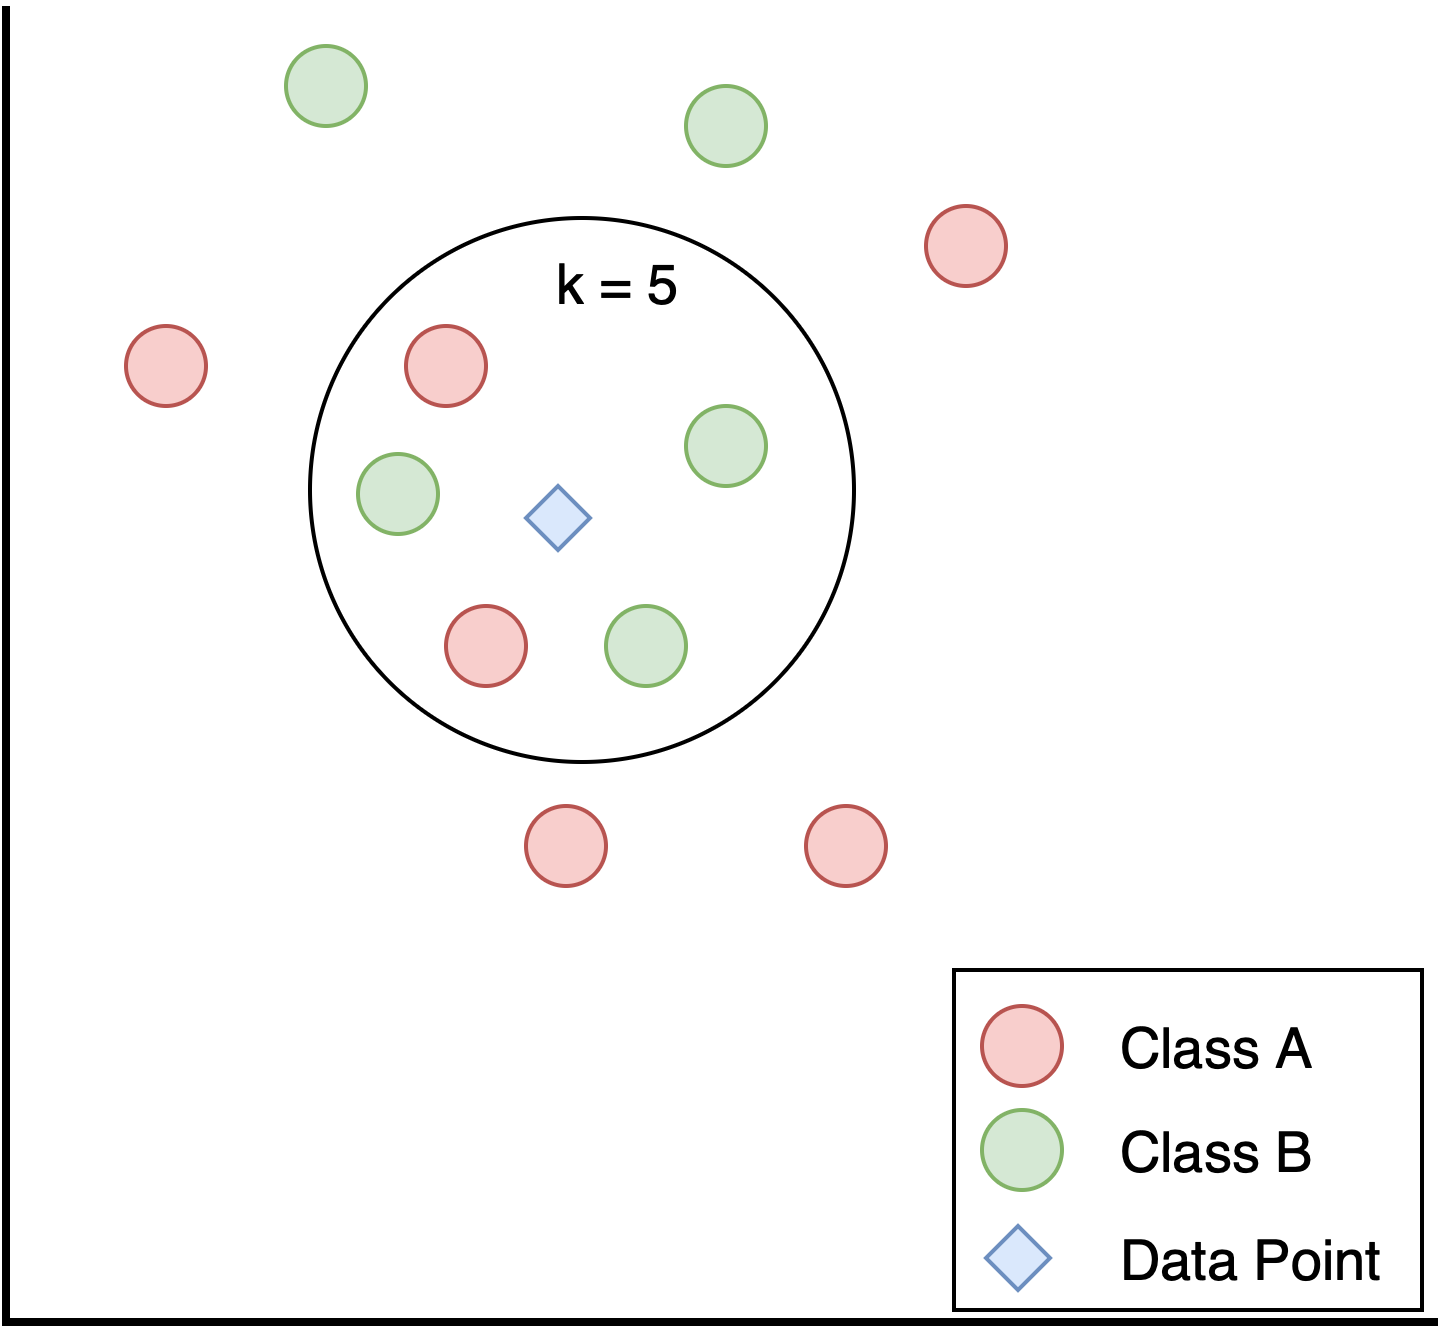
\includegraphics{graphics/classification/ClassificationKNeighbours.png}
    \caption{
    The target class for the data point when $k$ = 5 is Class B.
    }
    \label{fig:classification-knearestneighbours}
\end{marginfigure}

\begin{equation}\label{eq:euclideanDistance}
    d(x,y) = \sqrt{\sum_{i=1}^{n}(x_{i}-y_{i})^2}
\end{equation}

\begin{equation}\label{eq:manhattanDistance}
    d(x,y) = \sum_{i=1}^{n}|x_{i}-y_{i}|
\end{equation}

A \textit{distance function}\index{classification!k-nearest neighbour!distance function}, such as the \textbf{Euclidean distance} in equation~\ref{eq:euclideanDistance} or \textbf{Manhattan distance} in equation~\ref{eq:manhattanDistance}, is used to calculate the closest $k$ neighbours. In these equations, $x$ and $y$ refer to the two points between which the distance is to be calculated, $n$ is the number of features in the data points, and $x_i$ and $y_i$ are the values of the data points at the $i^{th}$ feature.

The effectiveness of the KNN classifier strongly depends on the $k$ value, which can be in the range [1, $n$], where $n$ is the number of samples. When 1 is chosen as the $k$ value, the unknown point takes the class of its nearest neighbour \citep{neelamegam2013}. Even though the value for $k$ is normally guessed, some may prefer referring to the following heuristics \citep{kirk2017} to determine their $k$:
\begin{itemize}
    \item Avoid choosing a large value for $k$
    \item In binary classifications, $k$ should ideally be an even number
    \item $k$ must equal or be greater than the number of classes plus one
\end{itemize}

\section{Multiclass Classification}
\label{sec:multiclass}
\index{classification!multiclass classification}

Multiclass classification models are able to determine a class for an unseen example from $k$ classes, where $k$ > 2. A multiclass classification problem may be solved by extending the aforementioned classification algorithms, and others including \textit{Neural Networks}\index{classification!multiclass classification!neural networks} and \textit{Support Vector Machines}\index{classification!multiclass classification!support vector machines} \citep{aly2005}. \citet{aly2005} discusses approaching a multiclass classification problem by decomposing it into multiple binary classification problems, which can then be solved using binary classifiers.

\subsection{One-versus-all (OVA)} \index{classification!multiclass classification!one-versus-all}
This approach considers $k$ binary classifiers, where $k$ is the number of classes. Each classifier is trained on data composed of positive examples from the $k^{th}$ class and negative examples from the remaining $k$-1 classes. Unseen examples are assigned the class of the classifier which obtains the highest output \citep{aly2005}.

\subsection{All-versus-all (AVA)} \index{classification!multiclass classification!all-vs-all}

In this approach, $\frac{k(k-1)}{2}$ binary classifiers are built to distinguish between all the possible pairs of classes. When predicting, all classifiers are considered and the class obtaining the highest score is taken as the target class \citep{aly2005}.\\

Apart from these two methods, \textit{Error-Correcting Output-Coding (ECOC)}\index{classification!multiclass classification!error-correcting output-coding} \citep{dietterich1995} and \textit{Generalized Coding}\index{classification!multiclass classification!generalized coding} \citep{allwein2001} may also be applied.

\index{classification|)}